\documentclass{report} 
\title{Strang}
\date{Started 5th June 2025}
\author{Malcolm}
\usepackage{amsmath} %import math
\usepackage{mathtools} %more math
\usepackage{amssymb} %for QED symbol
\usepackage{amsthm} %
\usepackage{bm}%bold math
\usepackage{graphicx} %import imaging
\graphicspath{{./images/}} %set imaging path
\begin{document}
\maketitle

\tableofcontents

\newpage

\chapter{Vectors and Matrices}
\section{Intuition for Dot product, Cosine formula, Schwarz and Triangle inequalities}
\textbf{Intuition for dot product}\\
The unit vectors $\bm{v}=(\cos\alpha,\sin\alpha)$ and $\bm{w}=(\cos\beta,\sin\beta)$ are plotted as follows
\begin{center}
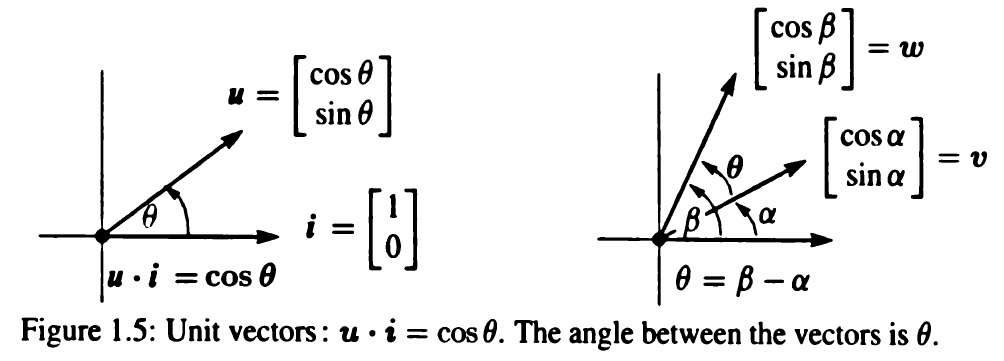
\includegraphics[width=10cm]{1}
\end{center}
See first that when fixed in this form, the magnitude of both vectors is 1, with an angle $\beta-\alpha$ between them. These unit vectors have dot product
\begin{equation*}
\bm{v}\cdot\bm{w}=\cos\alpha\cos\beta+\sin\alpha\sin\beta=\cos(\beta-\alpha)
\end{equation*}
We have $\theta$ as the angle between the two vectors; see that the sign of $\bm v\cdot\bm w$ tells us whether $\theta$ is below or above a right angle (due
to the cosine function being negative for its argument $>\pi/2$ and positive for $<\pi/2$):
\begin{center}
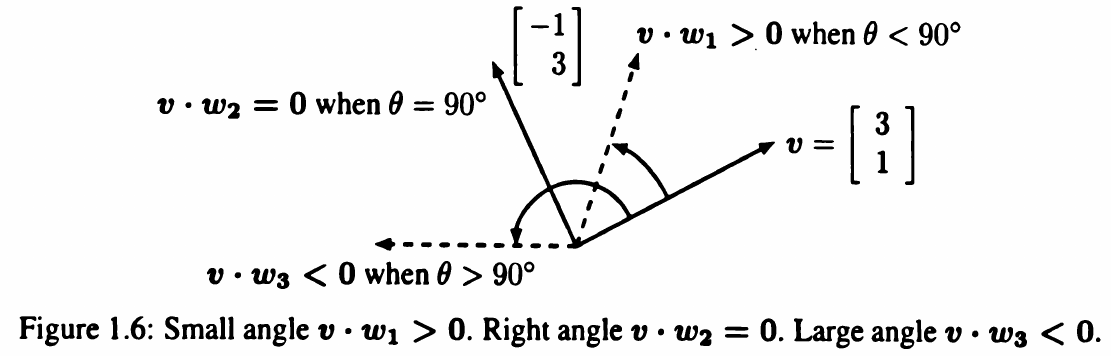
\includegraphics[width=9cm]{2}
\end{center}
(next page)\newpage
\noindent\textbf{Cont.}\\
The idea here is that the dot product reveals the exact angle $\theta$; for unit vectors $\bm u$ and $\bm U$, the dot product $\bm u\cdot\bm U$ is the cosine of 
$\theta$. Ths remains true in $n$ dimensions (not shown).\\
\vspace{1mm}\\
See that any $\bm{u}$ and $\bm{v}$ can be fixed in the above form by normalising their lengths to get
$\bm u=\bm v/||\bm v||$ and $\bm U=\bm w/||\bm w||$. After which their dot product would give $\cos\theta$. This leads us to the \textit{cosine formula}:
\begin{equation*}
\text{\textbf{Cosine formula}: }
\frac{\bm v\cdot\bm w}{||\bm v||\,||\bm w||}=\cos\theta\quad\text{ if $\bm v$ and $\bm w$ are nonzero vectors}
\end{equation*}
\textbf{Perpendicular vectors}\\
See that when the angle between $\bm v$ and $\bm w$ is $90^\circ$, its cosine is 0; this gives us a way to test this. Also see that for perpendicular vectors:
\begin{equation*}
||\bm v+\bm w||^2=||\bm v||^2+||\bm w||^2
\end{equation*}
because
\begin{equation*}
||\bm v+\bm w||^2=(\bm v+\bm w)\cdot(\bm v+\bm w)=\bm v\cdot\bm v+\bm v\cdot\bm w+\bm w\cdot\bm v+\bm w\cdot\bm w
\end{equation*}
where $\bm v\cdot \bm w=0$.\\
\vspace{1mm}\\
\textbf{Schwarz and Triangle inequalities}\\
First, see from the cosine formula that the dot product of $\bm v/||\bm v||$ and
$\bm w/||\bm w||$ never exceeds one (since $\cos\theta$ never exceeds one). This is the the 
\textit{Schwarz inequality}:
\begin{equation*}
\text{\textbf{Schwarz inequality}: }|\bm v\cdot\bm w|\leq||\bm v||\,||\bm w||
\end{equation*}
The \textit{Triangle inequality} comes directly from the Schwarz inequality:
\begin{equation*}
\text{\textbf{Triangle inequality}: }||\bm v+\bm w||\leq||\bm v||+||\bm w||
\end{equation*}
This can be seen from
\begin{equation*}
||\bm v+\bm w||^2=\bm v\cdot\bm v+\bm v\cdot\bm w+\bm w\cdot\bm v+\bm w\cdot\bm w
\leq||\bm v||^2+2||\bm v||\,||\bm w||+||\bm w||^2
\end{equation*}
The square root gives us the triangle equality (side 3 cannot exceed side 1 + side 2).
\newpage

\section{Intuition for column rank being equal to row rank}
If all columns are in the same direction, why does it happen that all the rows are the same direction?\\
\vspace{1mm}\\
Consider the matrix, see that column 2 is $m$ times column 1:
\begin{equation*}
\bm A=\left[\begin{array}{cc}
a&ma\\
b&mb
\end{array}\right]
\end{equation*}
See that the second row is just $b/a$ times the first row---if the column rank is 1, then the row rank is 1. See that transposing the matrix, we have
\begin{equation*}
\bm A=\left[\begin{array}{cc}
a(1)&b(1)\\
a(m)&b(m)
\end{array}\right]
\end{equation*}
which still has one independent column. Now consider the 3x3 case:
\begin{equation*}
\bm A=\left[\begin{array}{ccc}
a&ma&pa\\
b&mb&pb\\
c&mc&pc
\end{array}\right]
\end{equation*}
See that a similar deduction can also be made in this case, where the row rank of $A$ is equal to its column rank.\\
(next page)\newpage
\noindent\textbf{An informal proof}\\
Consider any matrix $\bm A$, suppose we go from left to right, looking for independent columns of $\bm A$ using the following procedure:
\begin{enumerate}
\item If column 1 of $\bm A$ is not zero, put it in matrix $\bm C$
\item If column 2 of $\bm A$ is not a multiple of column 1, put it in into $\bm C$
\item If column 3 of $\bm A$ is not a combination of columns 1 and 2, put it into $C$. \textit{continue}
\end{enumerate}
See that at the end $\bm C$ will have $r$ columns taken from $\bm A$, where $r$ is the rank of $\bm A$ and $\bm C$. While the $n$ columns of $\bm A$ are dependent, 
the $r$ columns of $\bm C$ will surely be independent.\\
\vspace{1mm}\\
For instance consider $\bm A$ with rank 2
\begin{equation*}
\bm A=\left[\begin{array}{ccc}
2&6&4\\
4&12&8\\
1&3&5
\end{array}\right]\quad\text{leads to}\quad \bm C=
\left[\begin{array}{cc}
2&4\\
4&8\\
1&5
\end{array}\right]
\end{equation*}
Now consider another matrix $\bm R$ to be multiplied by $\bm C$ such that 
$\bm A=\bm{CR}$. The first and third columns of $\bm A$ are already in $\bm C$, so those respective columns in $\bm R$ make up a \textit{identity matrix};
the second column of $\bm A$ is a multiple of the first, so we have
\begin{equation*}
\bm A=\bm{CR}\quad\text{is }\left[\begin{array}{ccc}
2&6&4\\
4&12&8\\
1&3&5
\end{array}\right]=
\left[\begin{array}{cc}
2&4\\
4&8\\
1&5
\end{array}\right]
\left[\begin{array}{ccc}
1&3&0\\
0&0&1
\end{array}\right]
\end{equation*}
(See that the $i$th row of $\bm A$ can be seen as a linear combination of the rows of $\bm R$ specified the $i$th row of $\bm C$. 
(or just consider $\bm A^T=\bm R^T\bm C^T$). We know that
\begin{enumerate}
\item $\bm C$ contains the full set of $r$ independent columns of $\bm A$.
\item $\bm R=[\bm{I\,\bm F}]$ contains the identity matrix $\bm I$ in the same $r$ columns that held $\bm C$.
\item The dependent columns of $\bm A$ are combinations of $\bm{CF}$ of the independent columns in $\bm C$.
\end{enumerate}
Where the matrix $\bm F$ goes into the other $n-r$ columns of $\bm R=[\bm{I\,\bm F}]$. ($\bm A=\bm{CR}$ becomes $\bm A=\bm{C[I,F]}=\bm{[C,CF]}=
[\text{indep cols of $\bm A$},\text{ dep cols of $\bm A$}]$ (in correct order).\\
\vspace{1mm}\\
See that $\bm C$ has the same column space as $\bm A$, and $\bm R$ \textit{has the same row space} as $\bm A$ (every row of $\bm A$ is a combination of the rows
of $\bm R$).\\
(next page)\newpage
\noindent\textbf{Cont.}\\
We had the example
\begin{equation*}
\bm A=\bm{CR}\quad\text{is }\left[\begin{array}{ccc}
2&6&4\\
4&12&8\\
1&3&5
\end{array}\right]=
\left[\begin{array}{cc}
2&4\\
4&8\\
1&5
\end{array}\right]
\left[\begin{array}{ccc}
1&3&0\\
0&0&1
\end{array}\right]
\end{equation*}
\textit{Here is an informal proof that the row rank of $\bm A$ equals the column rank of $\bm A$} (based from facts we already know)
\begin{enumerate}
\item The $r$ columns of $\bm C$ are independent (chosen that way from $\bm A$)
\item Every column of $\bm A$ is a combination of those $r$ columns of $\bm C$ (since $\bm A=\bm{CR}$)
\item The $r$ rows of $\bm R$ are independent (they contain the $r$ by $r$ matrix $\bm I$)
\item Every row of $\bm A$ is a combination of the $\bm r$ rows of $\bm R$
\end{enumerate}
See that for every column of $\bm A$ that goes into $\bm C$, a column of $\bm I$ goes into $\bm R$, where each column of $\bm I$ in $\bm R$ adds an independent row.\\
\vspace{1mm}\\
This means that the column rank of $\bm C$ (column space of $\bm A$) is always equal to the row rank of $\bm R$ (row space of $\bm A$)---the 
column rank of $\bm A$ is equal to the row rank of $\bm A$.\\
\vspace{1mm}\\
\textbf{More examples}\\
Rank 2:
\begin{equation*}
\left[\begin{array}{ccc}
1&2&3\\
4&5&6\\
7&8&9
\end{array}\right]=
\left[\begin{array}{cc}
1&2\\
4&5\\
7&8
\end{array}\right]
\left[\begin{array}{ccc}
1&0&-1\\
0&1&2
\end{array}\right]
\end{equation*}
Rank 2:
\begin{equation*}
\left[\begin{array}{cccc}
1&2&3&4\\
1&2&4&5
\end{array}\right]=
\left[\begin{array}{cc}
1&3\\
1&4
\end{array}\right]
\left[\begin{array}{cccc}
1&2&0&1\\
0&0&1&1
\end{array}\right]
\end{equation*}
Rank 1:
\begin{equation*}
\left[\begin{array}{cccc}
1&2&10&100\\
3&6&30&300\\
2&4&20&200
\end{array}\right]=
\left[\begin{array}{c}
1\\3\\2
\end{array}\right]
\left[\begin{array}{cccc}
1&2&10&100
\end{array}\right]
\end{equation*}
\newpage

\section{Ways to multiply $\bm{AB}=\bm C$}
\textbf{Multiplcation by columns of $\bm A$ and rows of $\bm B$}\\
A lesser known way to multiply $\bm{AB}$ is through considering the columns of $\bm A$ and the rows of $\bm B$ (contrary to the usual ideas where each 
entry of the result is a dot product of a row of $\bm A$ and column of $\bm B$):
\begin{center}
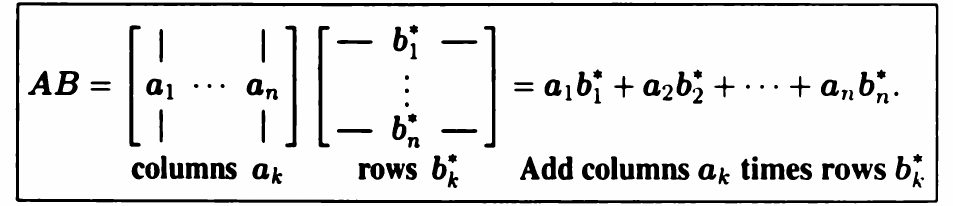
\includegraphics[width=10cm]{3}
\end{center}
We multiply each column of $\bm A$ by each row of $\bm B$; this gives us $n$ rank 1 matrices, which we then sum together; these matrices are called \textit{outer products}\\
\vspace{1mm}\\
(usually we see the $i$th column of the result as a linear combination of the columns of $\bm A$ specified by the $i$th column of $\bm B$. However
in this case the $i$th outer product is a matrix of the same size as the result, that contains all the contributions of the $i$th column of $\bm A$ to the final product.
By summing this over all $n$ columns of $\bm A$ we get the result.)\\
\vspace{1mm}\\
\textbf{Summary of methods}
\begin{center}
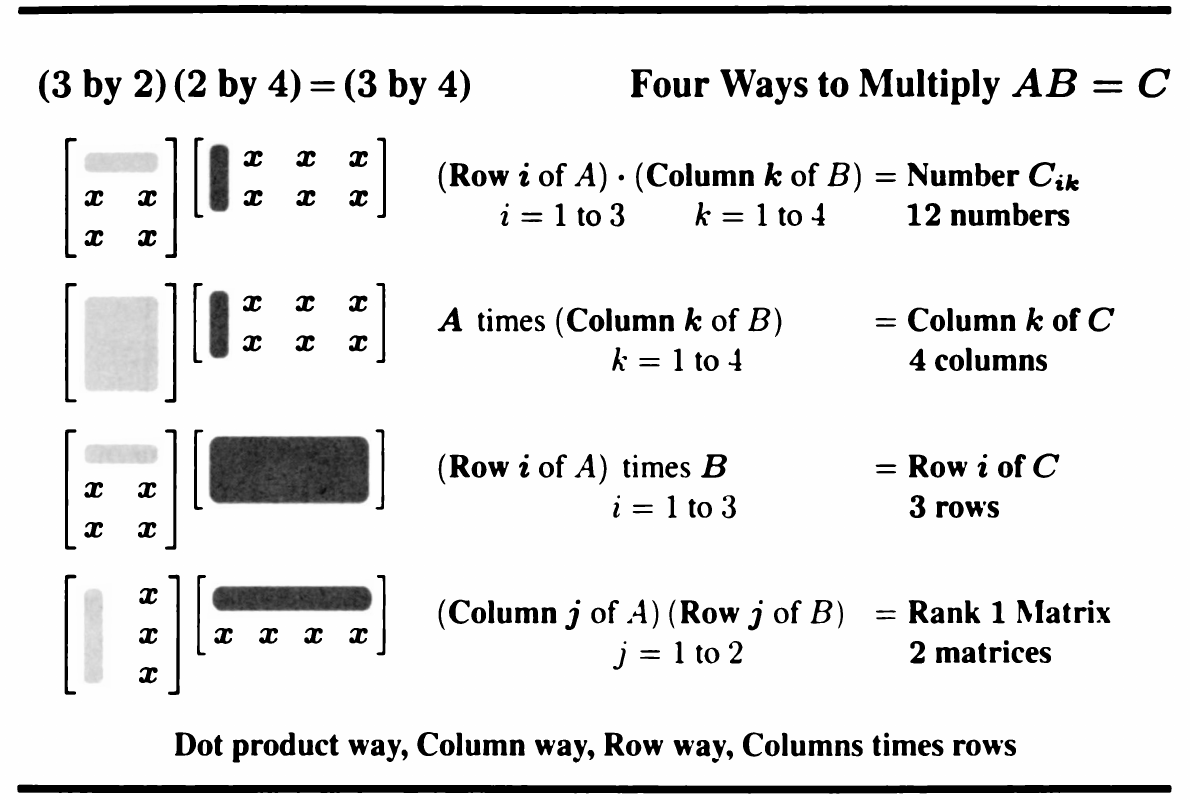
\includegraphics[width=10cm]{4}
\end{center}
(A nice way to intuit the the third method is to consider $(\bm{AB})^T=\bm B^T\bm A^T$; where the columns of $(\bm{AB})^T$ are the rows of $\bm{AB}$)
\newpage

\chapter{Solving linear equations $\bm{Ax}=\bm b$}\newpage

\section{Solutions to $\bm{Ax}=\bm b$}
Given a $n$x$n$ matrix $\bm A$ and an $n$x1 column vector $b$, there are three outcomes for the vector $\bm x$ that solves $\bm{Ax}=\bm b$.\\
\vspace{1mm}\\
First there may be \textit{no vector} $\bm x$ that solves $\bm{Ax}=\bm b$, or there may be exactly \textit{one} solution, or there may be \textit{infinitely many}
solution vectors $\bm x$. Here are the possibilities:\\
\vspace{1mm}\\
1. \textbf{Exactly one solution} to $\bm{Ax}=\bm b$ means that $\bm A$ has independent columns (only one particular linear combination of the columns of $\bm A$
leads to $\bm b$. That combination is specified by $\bm x$). $\bm A$ is full rank and the only solution to $\bm{Ax}=\bm{0}$ is $\bm x=\bm0$. 
$\bm A$ \textit{has an inverse matrix} $\bm A^{-1}$ (given $\bm b$, we can work backward to get $\bm x$ since only one $\bm x$ leads to $\bm b$).\\
\vspace{1mm}\\
2. \textbf{No solution} to $\bm{Ax}=\bm b$ means that $\bm b$ is not in the column space of $\bm A$, so $\bm A$ is not full rank.\\
\vspace{1mm}\\
3. \textbf{Infinitely many solutions}. See that when the columns of $\bm A$ are not independent (not full rank), then there are infinitely many ways to
produce the zero vector $\bm b=\bm0$ (this is the meaning of dependent columns), and so there are infinitely many solutions to $\bm{AX}=\bm0$.\\
\vspace{1mm}\\ 
Also see that if $\bm A$ is not full rank it means that its column space is some subspace, where
solutions only exist for $\bm b$ within that subspace.\\
\vspace{1mm}\\
As such, if there so happens to be a solution to $\bm{Ax}=\bm b$ then we can add any solution to $\bm{AX}=\bm0$:
\begin{equation*}
\bm A(\bm x+\alpha\bm X)=\bm A\bm x+\alpha\bm A\bm X=\bm b+\bm0=\bm b
\end{equation*}
For some constant $\alpha$, which gives us $\bm b$ again---we have infinitely many solutions.
\newpage

\section{Elimination and Back Substitution}
\textbf{Elimination}\\
We want to produce an \textit{upper triangular} matrix $\bm U$ from a square matrix $\bm A$. This is done through elimination; the procedure (for a 3x3 matrix) is as
follows (assuming no row exchanges):
\begin{enumerate}
\item Use the first equation(row) to produce zeros in column 1 below the first pivot.
\item Use the new second equation(row) to clear out column 2 below pivot 2 in row 2.
\item \textit{Continue to column 3}. The expected result is an upper triangular matrix $\bm U$.
\end{enumerate}
These steps can be carried out using elimination matrices $\bm E$.\\
\vspace{1mm}\\
Consider $\bm A$ and $\bm b$
\begin{equation*}
\bm A=\left[\begin{array}{ccc}
2&3&4\\
4&11&14\\
2&8&17
\end{array}\right]\quad
\bm b=\left[\begin{array}{c}
19\\55\\50
\end{array}\right]
\end{equation*}
$\bm E_{21}$ multiplies equation 1 by 2 and subtracts that from equation 2 to get a zero in the first column below the first pivot:
\begin{equation*}
\bm E_{21}=\left[\begin{array}{ccc}
1&0&0\\
-2&1&0\\
0&0&1
\end{array}\right]\implies
\bm E_{21}\bm A=\left[\begin{array}{ccc}
2&3&4\\
0&5&6\\
2&8&17
\end{array}\right],\quad
\bm E_{21}\bm b=\left[\begin{array}{c}
19\\17\\50
\end{array}\right]
\end{equation*}
(For intuition on the elimination matrices, consider the row perspective of matrix multiplication) This produced the desired zero in column 1. It changed equation 2.
To make the first pivot column zero, we subtract row 1 from row 3 using $\bm E_{31}$
\begin{equation*}
\bm E_{31}=\left[\begin{array}{ccc}
1&0&0\\
0&1&0\\
-1&0&1
\end{array}\right]\implies
\bm E_{31}\bm E_{21}\bm A=\left[\begin{array}{ccc}
2&3&4\\
0&5&6\\
0&5&13
\end{array}\right],\quad
\bm E_{31}\bm E_{21}\bm b=\left[\begin{array}{c}
19\\17\\31
\end{array}\right]
\end{equation*}
This completes elimination in column 1. Moving on to column 2 row 2 (the second pivot row). We use $\bm E_{32}$ to subtract equation 2 from equation 3
\begin{equation*}
\bm E_{31}=\left[\begin{array}{ccc}
1&0&0\\
0&1&0\\
0&-1&1
\end{array}\right]\implies
\bm U=\left[\begin{array}{ccc}
2&3&4\\
0&5&6\\
0&0&7
\end{array}\right],\quad
\bm c=\left[\begin{array}{c}
19\\17\\14
\end{array}\right]
\end{equation*}
$\bm E_{32}\bm E_{31}\bm E_{21}\bm A=\bm U$ is triangular. See that the same steps were applied to the right hand side 
$\bm b$ to produce a new right hand side $\bm c$.\\
(next page)\newpage
\noindent\textbf{Possible breakdown of elimination}\\
Elimination might fail. This occurs when zero appears in a pivot position---subtracting that zero from lower rows will not clear out the column
below that pivot. For example:
\begin{equation*}
\bm A=\left[\begin{array}{ccc}
2&3&4\\
4&6&14\\
2&8&17
\end{array}\right]\to
\left[\begin{array}{ccc}
2&3&4\\
0&0&6\\
0&5&13
\end{array}\right]=\bm B
\end{equation*}
A possible way to get around this would be to \textit{exchange} row 2 (with the zero pivot) for row (with the nonzero in that column), then carry out elimination
as per usual. This exchange is carried out using the permuation matrix $\bm P$:
\begin{equation*}
\bm{PB}=
\left[\begin{array}{ccc}
1&0&0\\
0&0&1\\
0&1&0
\end{array}\right]
\left[\begin{array}{ccc}
2&3&4\\
0&0&6\\
0&5&13
\end{array}\right]=
\left[\begin{array}{ccc}
2&3&4\\
0&5&13\\
0&0&6
\end{array}\right]
\end{equation*}
In this example the exchange produced $\bm U$ with nonzero pivots; normally there may be more columns eliminate before $\bm U$ is reached.\\
\vspace{1mm}\\
At times this exchange strategy may not work. This occurs when there is no pivot is available. Consider $\bm A'$:
\begin{equation*}
\bm A'=\left[\begin{array}{ccc}
2&3&4\\
4&6&14\\
2&3&17
\end{array}\right]\to
\left[\begin{array}{ccc}
2&3&4\\
0&0&6\\
0&0&13
\end{array}\right]=\bm U'
\end{equation*}
There is no second pivot in this case. This tells us that the matrix $\bm A'$ \textit{did not have full rank} (intuitively see that the non-pivot row can be expressed
as a linear combination of the other pivot rows, so the row space 
(which is equal to the row space of the original $\bm A'$ since the elimination steps are just linear combinations of the existing rows) 
is not full rank, and so the column space of the 
original $\bm A'$ is also not full rank.\\
\vspace{1mm}\\
In this case there will be nonzero solutions $\bm X$ to $\bm A'\bm X=0$. The columns of $\bm U'$ (and $\bm A'$) are not independent.\\
\vspace{1mm}\\
\textbf{Augmented matrix}\\
During elimination, in order to make sure that the operations on the matrix $\bm A$ are also executed on $\bm b$, one can 
\textit{include $\bm b$ as an extra column of $\bm A$}; this combination $[\bm A,\bm b]$ is called an \textit{augmented matrix}:
\begin{equation*}
\left[\begin{array}{cc}\bm A&\bm b\end{array}\right]=
\left[\begin{array}{cccc}
2&3&4&19\\
4&11&14&55\\
2&8&17&50
\end{array}\right]\xrightarrow{E}
\left[\begin{array}{cccc}
2&3&4&19\\
0&5&6&17\\
0&0&7&14
\end{array}\right]=
\left[\begin{array}{cc}\bm U&\bm c\end{array}\right]
\end{equation*}
(next page)\newpage
\noindent\textbf{Back Substitution to solve $\bm{Ux}=\bm c$}\\
Elimination (ideally) produces an upper triangular matrix $\bm U$ that has all zeros below the diagonal, with nonzero pivots. For instance we had, for some $\bm x$
\begin{equation*}
\bm{Ax}=\bm b,\quad\bm A=\left[\begin{array}{ccc}
2&3&4\\
4&11&14\\
2&8&17
\end{array}\right]\quad
\bm b=\left[\begin{array}{c}
19\\55\\50
\end{array}\right]
\end{equation*}
undergo elimination to to become
\begin{equation*}
\bm{Ux}=\bm c,\quad\bm U=\left[\begin{array}{ccc}
2&3&4\\
0&5&6\\
0&0&7
\end{array}\right]\quad
\bm c=\left[\begin{array}{c}
19\\17\\14
\end{array}\right]
\end{equation*}
See that this form allows us to easily solve the equations by going from bottom to top in a procedural manner, finding $x_3$, then $x_2$, then $x_1$:
\begin{enumerate}
\item\textit{Back substitution}: The last equation $7x_3=14$ gives $x_3=2$
\item\textit{Work upwards}: The next equation $5x_2+6(2)=17$ gives $x_2=1$
\item\textit{repeat}: The first equation $2x_1+3(1)+4(2)=19$ gives $x_1=4$
\end{enumerate}
giving us the only solution to this example $\bm x=(4,1,2)$. Remember the pivots need to be nonzero(full rank) for a single specific solution to be found.
\newpage

\section{Elimination matrices and inverse matrices}
\textbf{Elimination matrices}\\
The basic elimination step \textit{subtracts} a multiple $\ell_{ij}$ of equation $j$ from equation $i$. We always speak about \textit{subtractions} as elimination 
proceeds. For instance even if the first pivot $a_{11}=3$ and below it is
$a_{21}=-3$ where we could just add equation 1 to 2, we \textit{subtract} $\ell_{21}=-1$ \textit{times equation 1 from equation 2} (which gives
us the same result).\\
\vspace{1mm}\\
For instance here is the matrix that subtracts 2 times row 1 from row 3:
\begin{equation*}
\bm E_{31}=\left[\begin{array}{ccc}
1&0&0\\0&1&0\\-2&0&1\end{array}\right]
\end{equation*} 
If no row exchanges are needed, then three elimination matrices $\bm E_{21},
\bm E_{31},\bm E_{32}$ will produce three zeros below the diagonal to change $\bm A$ to the upper triangular $\bm U$(this just carries out elimination 
using matrices to represent each step).\\
\vspace{1mm}\\
\textbf{Inverse}\\
See that the \textit{inverse} of each matrix $\bm E_{ij}$ just \textit{adds back} $\ell_{ij}\,\cdot$ (row $j$) to row $i$. 
This leads to the inverse of their product $\bm E=\bm E_{32}\bm E_{31}\bm E_{21}$. We denote the inverse of $\bm E$ by $\bm L$. 
For instance, say some $\bm E$ subtracts 5 times row 1 from row 2, then $\bm E^{-1}$ adds 5 times row 1 to row 2:
\begin{equation*}
\bm E=\left[\begin{array}{ccc}
1&0&0\\-5&1&0\\0&0&1\end{array}\right],\quad
\bm E^{-1}=\left[\begin{array}{ccc}
1&0&0\\5&1&0\\0&0&1\end{array}\right]
\end{equation*}
(See that sequential application of these matrices, in either order, to some vector leads to no net change---as if we had multiplied by the identity.)\\
\vspace{1mm}\\
Now lets consider $\bm F$ which subtracts 4 times row 2 from row 3 (which might be a next step during elimination), naturally $\bm F^{-1}$ adds it back:
\begin{equation*}
\bm F=\left[\begin{array}{ccc}
1&0&0\\0&1&0\\0&-4&1\end{array}\right],\quad
\bm F^{-1}=\left[\begin{array}{ccc}
1&0&0\\0&1&0\\0&4&1\end{array}\right]
\end{equation*}
During elimination we would first apply $\bm E$ then $\bm F$, which is the same as applying $\bm{FE}$. Reversing the elimination would amount to 
$(\bm{FE})^{-1}$, which is the same as applying $\bm E^{-1}\bm F^{-1}$:
\begin{equation*}
\bm F\bm E=\left[\begin{array}{ccc}
1&0&0\\-5&1&0\\20&-4&1\end{array}\right]\quad\text{is inverted by}\quad
\bm E^{-1}\bm F^{-1}=\left[\begin{array}{ccc}
1&0&0\\5&1&0\\0&4&1\end{array}\right]
\end{equation*}
See that the product $\bm{FE}$ contains `20' but its inverse doesn't. In $\bm{FE}$, row 3 feels an effect of size 20 from row 1. However in $\bm E^{-1}\bm F^{-1}$ 
that doesn't happen.\\
(next page)\newpage
\noindent\textbf{$\bm L$ is the inverse of $\bm E$}\\
$\bm E$ is the product of all the elimination matrices $\bm E_{ij}$, it turns $\bm A$ into its upper triangular form $\bm{EA}=\bm U$ (assuming no row exchanges). 
The difficulty with $\bm E$ is multiplying all the separate elimination steps $\bm E_{ij}$ does not produce a good formula; illustrating 
$\bm E=\bm E_{32}\bm E_{31}\bm E_{21}$:
\begin{center}
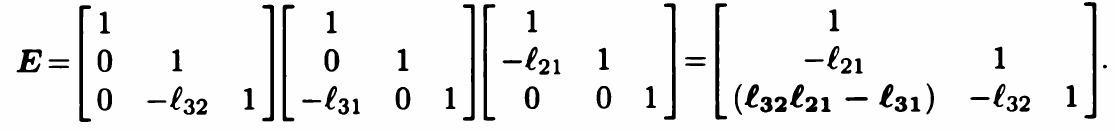
\includegraphics[width=10cm]{5}
\end{center}
See that the bottom left corner is dependent on multiple constants (since mutating the third row requries knowledge of the mutations that already occured to the
second row).\\
\vspace{1mm}\\
Now consider the inverse $\bm E^{-1}_{21}\bm E^{-1}_{31}\bm E^{-1}_{32}=\bm E^{-1}=\bm L$ (see that inverses need to be applied in reverse):
\begin{center}
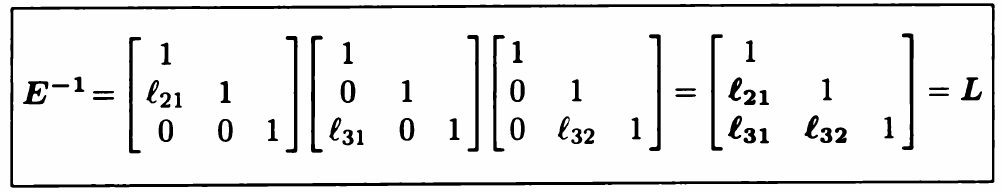
\includegraphics[width=10cm]{6}
\end{center}
(In the inverse matrix, the mutation of each row doesn't depend on previous mutations, so the multipliers fall into place in the lower triangular $\bm L$. 
Also see that the final matrix is only lower triangular because the elimination algorithm specifies that we don't manipulate the first row, and that we don't
manipulate the second row with the third row.)\\
\vspace{1mm}\\
This is why we might want to consider $\bm A=\bm{LU}$ to go back from triangular $\bm U$ to the original $\bm A$.
\newpage

\section{Gauss-Jordan elimination}
How would one compute the inverse of an $n$x$n$ matrix $\bm A$? Before answering that question, one might want to consider whether it is really necessary to know
$\bm A^{-1}$; although it is possible to find the solution to $\bm{Ax}=\bm b$ using $\bm x=\bm A^{-1}\bm{b}$, computing $\bm A^{-1}$ and taking $\bm A^{-1}\bm b$ is
a very slow way to find $\bm x$.\\
\vspace{1mm}\\
Say we want to compute $\bm A^{-1}$. This is equivalent to solving for $\bm{AX}=\bm I$. In that sense, by performing the manipulations on $\bm A$ to make it look
like $\bm I$. We essentially replicate the effect of $\bm A^{-1}$ on $\bm A$; by repeating those steps on the identity, 
it becomes as if we were taking $\bm A^{-1}\bm I=\bm A^{-1}$, allowing us to obtain the desired matrix.\\
\vspace{1mm}\\
This whole process can be done with an augmented matrix using \textit{Gauss-Jordan elimination}, where we essentially take steps to reduce $\bm A$ to reduced row
echelon form, while repeating said steps on the identity to obtain the inverse:
\begin{center}
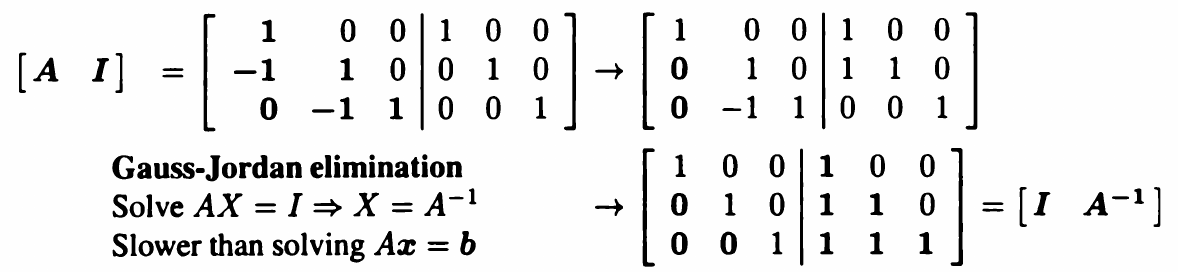
\includegraphics[width=10cm]{7}
\end{center}
The Gauss-Jordan essentially turns $[\bm A,\bm I]$ into $[I,\bm A^{-1}]$, where the elimination steps are essentially equivalent to multiplicaiton by $\bm A^{-1}$.
\newpage

\section{Proving $\bm A=\bm{LU}$}
Elimination is expressed by $\bm{EA}=\bm U$ and inverted by $\bm{LU}=\bm A$. It starts with $\bm A$ and ends with upper triangular $\bm U$, with each elimination step
being carried out by elimination matrices $\bm E_{ij}$. To invert one elimination step we add rows instead of subtracting:
\begin{center}
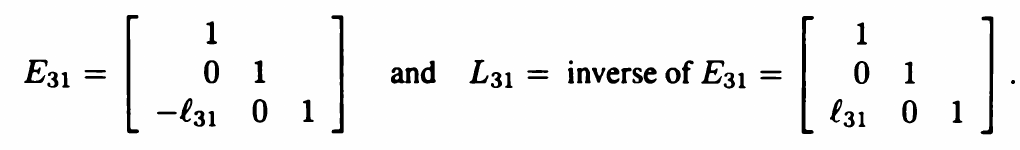
\includegraphics[width=10cm]{8}
\end{center}
Recall that $\bm E=\bm E_{32}\bm E_{31}\bm E_{21}$ gives us a fairly messy result:
\begin{center}
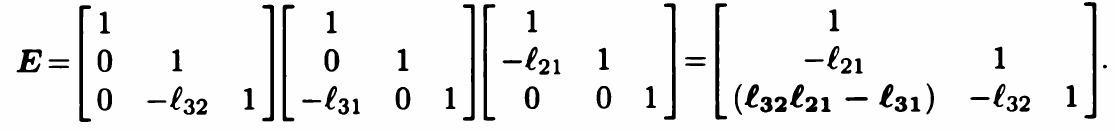
\includegraphics[width=10cm]{5}
\end{center}
while the inverse, $\bm E^{-1}=\bm E_{21}^{-1}\bm E_{31}^{-1}\bm E_{32}^{-1}=\bm L$ produces a much simpler result
\begin{center}
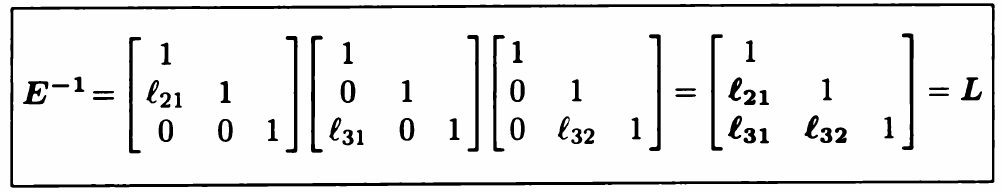
\includegraphics[width=10cm]{6}
\end{center}
We then have a elegant expression in $\bm A=\bm E^{-1}\bm U=\bm{LU}$. We now show that this equation holds over larger matrices of size $n$.\\
\vspace{1mm}\\
\textbf{Proof 1}\\
Following each step in elimination, consider the pivot rows that are subtracted from lower rows; see that these rows are not original rows of $\bm A$, since
they have been mutated by the previous elimination steps; they are instead rows of $\bm U$.\\
\vspace{1mm}\\
When computing the, say, third row of $\bm U$, we subtract multiples of earlier rows of $\bm U$:
\begin{equation*}
\text{Row 3 of $\bm U$}=(\text{Row 3 of $\bm A$})-\ell_{31}(\text{Row 1 of $\bm U$})-\ell_{32}(\text{Row 2 of $\bm U$})
\end{equation*}
Rewriting, see that
\begin{equation*}
\text{Row 3 of $\bm A$}=\ell_{31}(\text{Row 1 of $\bm U$})+\ell_{32}(\text{Row 2 of $\bm U$})+1(\text{Row 3 of $\bm U$})
\end{equation*}
Row $[\ell_{31},\ell_{32},1]$ is multiplying the matrix $\bm U$. This is \textit{exactly row 3 of $\bm A=\bm{LU}$}. All rows look like this regardless of the size of
$\bm A$. With no row exchanges, we have $\bm A=\bm{LU}$.\\
(next page)\newpage
\noindent\textbf{Proof 2}\\
Here is another proof. The idea here is to see elimination as removing one rank 1 matrix at a time---one column of $\bm L$ times one row of $\bm U$ from $\bm A$; 
where the problem becomes one size smaller with each iteration.\\
\vspace{1mm}\\
Elimination begins with pivot row = row 1 of $\bm A$. We multiply that pivot row by the numbers $\ell_{21}$, then $\ell_{31}$, and eventually $\ell_{n1}$; we subtract
the respective products from row 2, row 3, and eventually row $n$ of $\bm A$.
By choosing $\ell_{21}=a_{21}/a_{11}$, $\ell_{31}=a_{31}/a_{11}$ and so on until
$\ell_{n1}=a_{n1}/a_{11}$; now consider
if we also subtracted away the pivot row away from itself---this subtraction leaves zeros in column 1:
\begin{center}
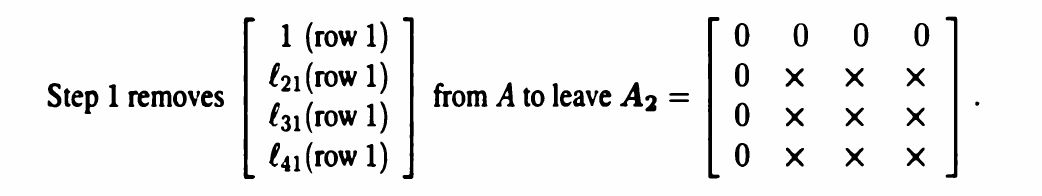
\includegraphics[width=10cm]{9}
\end{center}
The idea here is that we \textit{removed a rank 1 matrix} with columns made up of multiples of $\bm\ell_1=(1,\ell_{21},\ell_{31},\ell_{41},\ldots)$, 
scaled by
each respective entry of the first row of $\bm A$, which is also the first pivot row $\bm u_1$ of the final upper triangular matrix.\\
\vspace{1mm}\\
We continue with elimination in the second pivot column, using the second row as the pivot row; as before we also subtract the second pivot row from itself. 
See that this is again equivalent to subtracting a rank 1 matrix with basis
$\bm\ell_2=(0,1,\ell_{32},\ell_{42},\ldots)$. Recall that the second pivot row is the second row of the upper triangular matrix $\bm U$ in our factorisation.
\begin{center}
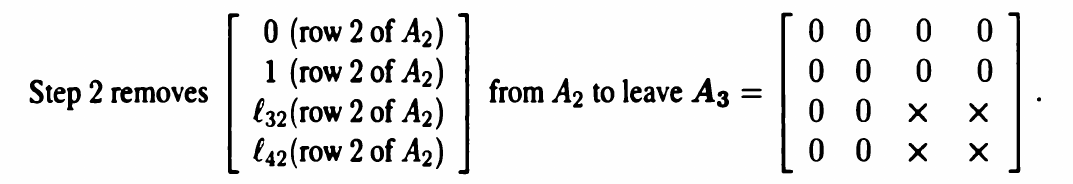
\includegraphics[width=10cm]{10}
\end{center}
Notice that both $\bm\ell_1$ and $\bm\ell_2$ are columns of $\bm L$.
We removed a column $\bm\ell_2$ times the second pivot row. Continuing in the same way, we successively remove columns with each step removing a column
$\bm\ell_j$ of $\bm L$ times a pivot row $\bm u_j$ of $\bm U$. See that this entire process can be depicted as
\begin{center}
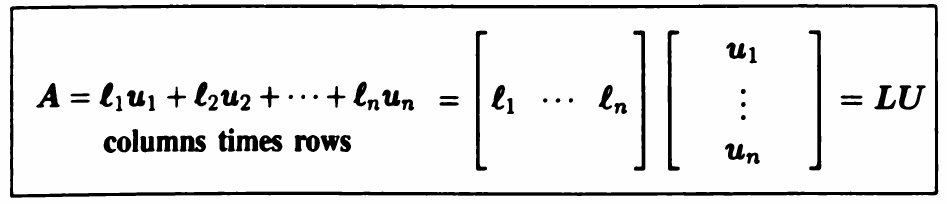
\includegraphics[width=10cm]{11}
\end{center}
Notice that $\bm U$ is upper triangular; the pivot row $u_k$ begins with $k-1$ zeros. $\bm L$ is lower triangular with 1's on the main diagonal. Column 
$\bm\ell_k$ also begins with $k-1$ zeros. (See that this proof makes use of the
idea that matrix multiplication can be seen as a sum of rank 1 matrices)
\newpage

\section{Permutation matrices}
\textbf{Examples}\\
Permutation matrices have a 1 in every row and a 1 in every column. All other entries are 0. When this matrix $\bm P$ multiplies a vector, it changes the order of 
its components; for instance:
\begin{center}
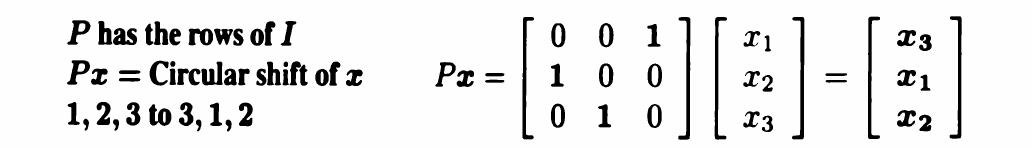
\includegraphics[width=10cm]{12}
\end{center}
(A nonzero $i$th entry on row $m$ of $\bm P$ means that row $i$ of $\bm x$ goes on that row $m$ in the result) Other examples include
\begin{center}
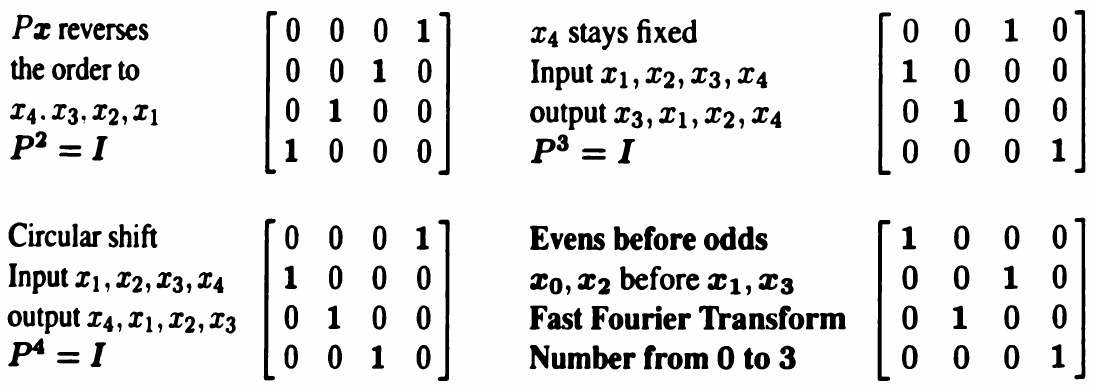
\includegraphics[width=10cm]{13}
\end{center}
Recall that elimination may require row exchanges. If $\bm A$ is invertible, then there is a permuation $\bm P$ to order its rows in advance, so that elimination
on $\bm{PA}$ meets no zeros in the pivot positions. Then $\bm{PA}=\bm{LU}$.\\
\vspace{1mm}\\
\textbf{Inverse}\\
We can intuit that the inverse of $\bm P$ is just its transpose:
\begin{center}
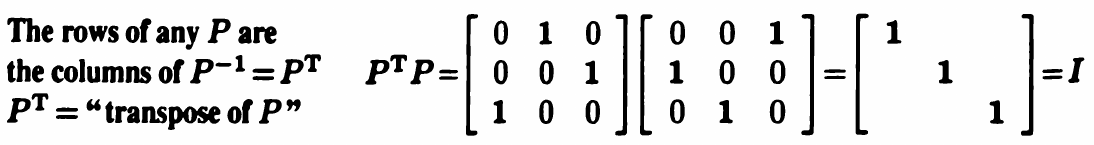
\includegraphics[width=10cm]{14}
\end{center}
(For instance, a nonzero entry in row 1 column 2 means `row 2 of $\bm x$ becomes row 1 of result'. Its transpose corresponds to a nonzero entry in 
row 2 column 1, so `row 1 of $\bm x$ becomes row 2 in the result'---reversing the change. This logic can be extrapolated to every other row.)\\
(next page)\newpage
\noindent\textbf{$\bm{PA}=\bm{LU}$ factorisation}\\












\end{document}
